\subsection{State-Space Models}

	Here, we present the State-Space Models (SSMs) (also known as Linear Dynamical Systems) based on Kevin Murphy's book \cite[Chapter 18]{mlBook} and Prof. Zoubin Ghahramani's paper \cite{ghahramani2000variational}. SSMs allow us to model systems that are dynamic. Unlike the SVMs, SSMs will model dependencies of the current state on the previous ones.
	
	\begin{figure}[h!]
		\centering
			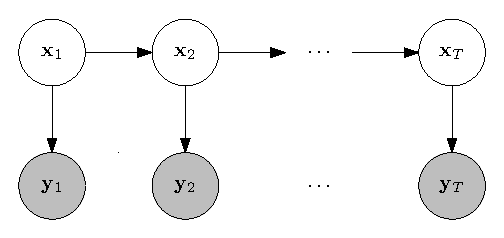
\includegraphics{drawings/pgm.eps}
		\caption{Probabilistic Graphical Model of a SSM and a HMM}
		\label{fig:pgm}
	\end{figure}
	
	We have two set of random variables, the hidden states $\left\{ \vec{x}_t,\vec{x}_t \in \mathbb{R}^d \right\}_{t = 1}^{T}$ and the observed vectors $\left\{ \vec{y}_t, \vec{y}_t \in \mathbb{R}^k \right\}_{t = 1}^{T}$. We can represent SSMs graphically in Figure \ref{fig:pgm}, and write out the joint probability of the model as
	\begin{equation}
		p\left( \left\{ \vec x_t, \vec y_t \right\}_{t = 1}^{T} \right) = p(\vec x_1) p(\vec y_1 | \vec x_1) \prod_{t = 2}^{T} {p(\vec x_t | \vec x_{t - 1}) p(\vec y_t | \vec x_t)}
	\end{equation}
In our case, we consider these particular transition and observation models with zero-mean Gaussian noises:
	\begin{align}
		\vec x_t & = \vec A \vec x_{t - 1} + \vec w_t\\
		\vec y_t & = \vec C \vec x_t + \vec v_t \\
		\vec w_t & \sim \mathcal{N} (\vec 0, \vec Q) \\
		\vec v_t & \sim \mathcal{N} (\vec 0, \vec R)
	\end{align}
Since we assume that $\pi = p(\vec x_1)$ is also Gaussian, all our conditional probability distributions will be Gaussian due to the linearity of the transition and observation models. Once the parameters are obtained, the problem of inference and state estimation consists of	
	\begin{enumerate}
		\item \textbf{Filtering.} We want to find $p(\vec x_t | \{\vec y_t\}_1^t)$. This is solved by the Kalman filtering algorithm.
		\item \textbf{Smoothing.} We want to find $p(\vec x_t | \{\vec y_T\}_1^t)$. This is solved by the Kalman smoothing algorithm.
		\item \textbf{Prediction.} We want to find $p(\vec x_{t + \tau} | \{\vec y_t\}_1^t)$. This is done by solving to 1. and then simulating using the state transition function.
	\end{enumerate}
We are mainly interested in filtering and smoothing.

\subsubsection{Our problem}
	Although SSMs are well-suited for time-series data, they are not very well suited for our problem because the hidden state $\vec x_t$ in this model is continuous, whereas in our problem, the sleeper's state is binary. While there are techniques to map from a continuous domain to a discrete one, we move on to discuss a more promising model.